\documentclass[english,output=paper,colorlinks,citecolor=brown]{../langscibook} 
\author{Nicolas Mazziotta\affiliation{Université de Liège}}
%\ORCIDs{}

\title{Grammar and graphical semiotics in early syntactic diagrams: Clark (1847) and Reed-Kellogg (1876)}
\shorttitlerunninghead{Grammar and graphical semiotics in early syntactic diagrams}
\abstract{This paper shows that the authors who first used diagrams to represent syntactic structures chose graphical conventions that constrained the way they could represent their analyses. Some graphical conventions may look similar despite following different rationales. Conversely, they may also look different and yet be grounded in the same logic. This second possibility becomes obvious when comparing the diagramming systems proposed by Clark (who uses aggregated bubbles) and Reed \& Kellogg (who use strokes). Nevertheless, bi-dimensional objects such as bubbles offer more varied layout possibilities for drawing diagrams than mono-dimensional objects such as strokes do. Consequently, authors have to add the representation for abstract concepts such as inclusion by means that are compatible with the basic objects they use.}

\IfFileExists{../localcommands.tex}{
  % add all extra packages you need to load to this file  

\usepackage{tabularx,multicol} 
\usepackage{url} 
\urlstyle{same}

\usepackage{listings}
\lstset{basicstyle=\ttfamily,tabsize=2,breaklines=true}

\usepackage{./langsci/styles/langsci-optional}
\usepackage{./langsci/styles/langsci-lgr}
\usepackage{./langsci/styles/langsci-gb4e}

  \newcommand*{\orcid}{}
\newcommand*{\markindex}{}

  %% hyphenation points for line breaks
%% Normally, automatic hyphenation in LaTeX is very good
%% If a word is mis-hyphenated, add it to this file
%%
%% add information to TeX file before \begin{document} with:
%% %% hyphenation points for line breaks
%% Normally, automatic hyphenation in LaTeX is very good
%% If a word is mis-hyphenated, add it to this file
%%
%% add information to TeX file before \begin{document} with:
%% %% hyphenation points for line breaks
%% Normally, automatic hyphenation in LaTeX is very good
%% If a word is mis-hyphenated, add it to this file
%%
%% add information to TeX file before \begin{document} with:
%% \include{localhyphenation}
\hyphenation{
affri-ca-te
affri-ca-tes
dis-ci-plin-ary
}

\hyphenation{
affri-ca-te
affri-ca-tes
dis-ci-plin-ary
}

\hyphenation{
affri-ca-te
affri-ca-tes
dis-ci-plin-ary
}

  \bibliography{../localbibliography}
  \togglepaper[4]%%chapternumber
}{}

\begin{document}
\maketitle

\section{Introduction}\label{sec:4:1}

This paper focuses on the graphical depiction of syntactic analysis. I will compare two early diagramming systems in order to show how graphical formalisms put constraints on what can be expressed, because of the spatial properties of the graphical units. I will focus on two aspects: how graphical devices represent linguistic units and how these graphical devices interact on the plane. The diagrams under study were created in the United States, and date from the 19th century \citep{Brittain1973}, thus preceding the advent of modern syntactic trees that are in use today. The introduction of syntactic diagrams occurred at a time when grammatical description in America had undergone a paradigm shift from word-centric to syntactic analysis.\footnote{\textrm{\citet[76]{AartsMcMahon2006}. Arguably, such a paradigm-shift is already achieved in the works of several French scholars at the beginning of the 18th century (see \citealt{ImrenyiMazziotta2020})}} Scholars began to focus on the “deep structure” of the \is{sentence}sentence. Pioneers made extensive use of diagrams to encode the structural order of syntactic relations and discarded the linear succession of words. 

In \sectref{sec:4:2}, I will introduce the formal and semiotic concepts that I use to describe the diagrams. In \sectref{sec:4:3}, I will present early diagramming systems, especially the ones produced by Stephen W. Clark (1810–1901) on the one hand, and Alonzo Reed (d.~1899) and Brainerd Kellogg (1834–1920) on the other hand. \sectref{sec:4:4} compares the graphical representation of three specific structures in these two systems.

\section{Visual depictions of syntax}\label{sec:4:2}

Visual depictions of syntactic analyses are diagrams, i.e., icons that represent relations and allow for creative thinking (\citealt{Peirce1994}, cf. \citealt[36--42]{Chauvire2008}). Syntactic diagrams represent words and grammatical concepts, and depict the way they interact. Since words and grammatical concepts are just \textit{thoughts} (albeit highly organized ones), they cannot be expressed without a way of making them perceptible. Syntactic diagrams achieve this goal by graphical means. In \sectref{sec:4:2.1}, I introduce the concepts of \textit{reification}, \textit{graphical entities} and \textit{spatial configurations}, which I rely on to describe the way linguistic analyses are graphically represented. \sectref{sec:4:2.2} illustrates the variety of diagrams. 

\subsection{\textit{Semiotic concepts}: Reification, graphical entities, spatial configurations}\label{sec:4:2.1}

To begin with, let us consider \figref{fig:4:1}, depicting a classical immediate constituent analysis (“ICA”) of \REF{ex:4:1}.\footnote{The sentence is taken from \citet[44]{Clark1870} for comparison purposes, but the analysis is mine. It should be noted that the diagram depicts a simple ICA in order to illustrate the grounding rationales of such a representation for comparison purposes. \figref{fig:4:1} is not seen here as a state of the art representation.} 

\ea \label{ex:4:1}%1
The fur warms a bear.
\z

\begin{figure}
    \begin{forest}
      [S
        [NP [the] [fur]]
        [VP [warms] [NP [a] [bear]]]
      ]
    \end{forest}
     \caption{Sample ICA tree\label{fig:4:1}}
\end{figure}

Each word is represented by itself (by self-reference) in the form of concatenated letters. Conceptual units such as constituents are represented in the same way. On the other hand, strokes represent part-whole relations. I call \textit{reification} such a discrete representation of a concept (\textit{to reify} ‘to turn into an object’; \citealt{KahaneMazziotta2015}). When a concept is reified in a graphical environment, it becomes a \textit{graphical entity} (\citealt{Groupe-µ1992}), i.e.~a sign that we are able to perceive, to delimit, and to describe from a visual point of view. Graphical entities are thus bound to conceptual units.

Graphical entities interact with one another by forming spatial \textit{configurations}: in \figref{fig:4:1}, one can understand that \textit{warms} and the second NP are immediate constituents of VP because they are both placed below VP, and they are each connected to VP by a stroke.\footnote{For the sake of simplicity, unless otherwise stated, I will use shortcuts such as “NP” for “the graphical entity that reifies NP”.} Spatial configurations express conceptual relations in the diagram.

\subsection{Variety in the graphical representation of analyses}\label{sec:4:2.2}

It is well known that there are various ways to represent the relations between words. The same conceptual units/relations can be reified in different ways. Moreover, graphical entities and spatial configurations are competing means of expressing analyses of the same kind. To illustrate this, I will compare the two diagrams in \figref{fig:4:2}: (a) is the very first syntactic diagram, proposed by Gustav Billroth (1808–1836) in \citeyear{Billroth1832} (the analysed sentence can be literally translated as: `Miltiades, leader of the Athenians, restored nearly suppressed freedom to the entire Greece, in the battle at Marathon'); (b) is a diagram from \textit{Graded lessons in English} (\citeyear{ReedBrainerd1879}) by Alonzo Reed and Brainerd Kellogg.

\begin{figure}
	\caption{Various values of strokes\label{fig:4:2}}
	\begin{subfigure}[t]{\linewidth}\centering
	\caption{\label{fig:4:2a}\citealt[102]{Billroth1832}}
	  	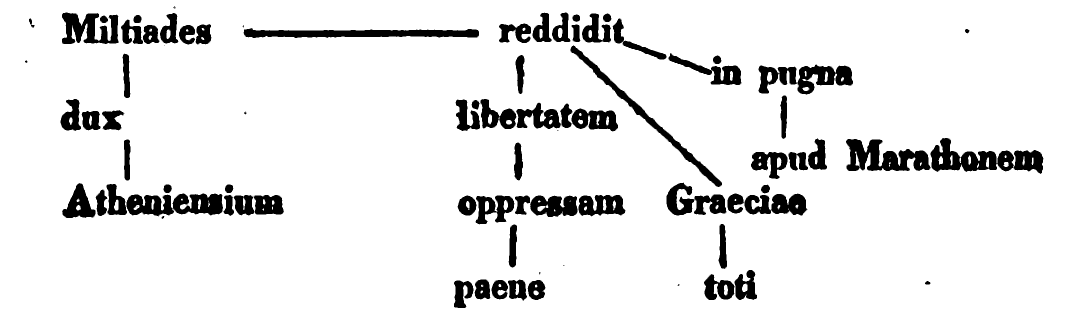
\includegraphics[width=.75\textwidth]{figures/04/Billroth.png}
        \end{subfigure}\medskip\\%
        \begin{subfigure}[t]{\linewidth}\centering
		\caption{\label{fig:4:2b}\citealt[62]{ReedBrainerd1879}}
		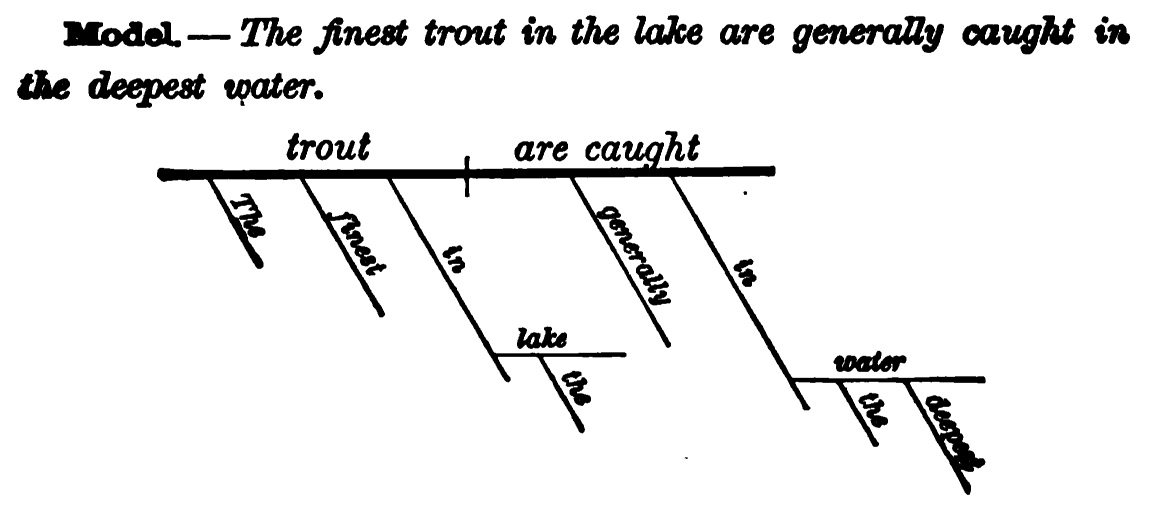
\includegraphics[width=.75\textwidth]{figures/04/ReedKellog.png}
	\end{subfigure}
\end{figure}

Despite the fact that both diagrams represent words and the way they interact in the sentence, and despite the fact that both diagrams make use of concatenated characters and strokes, their rationales are very different. In \figref{fig:4:2}a, words are reified by concatenated characters, whereas in \figref{fig:4:2}b, words are reified by a combination of concatenated characters and strokes below them, i.e.~\textit{labeled strokes}. Both diagrams express how words are grouped into larger structures, such as phrases and sentences. In \figref{fig:4:2}a, strokes reify the grouping of words in a way that we are very accustomed to: many diagrams of all sorts use similar conventions. On the contrary, unless we learned to read \figref{fig:4:2}b at school, it takes a while to get accustomed to the fact that strokes in \figref{fig:4:2}b do not reify syntactic relations as they do in \figref{fig:4:2}a. Actually, in \figref{fig:4:2}b, relations are mostly represented by the relative positions of the words, i.e., by spatial configurations.

This comparison demonstrates two important features of graphical entities. Firstly, they are complete signs with a specific form of expression and a value: using the same form of expression does not automatically entail that the same value is implied, and \textit{vice versa}. The configurational properties of the entities differ accordingly: in \figref{fig:4:2}a, strokes are drawn \textit{between} words, whereas in \figref{fig:4:2}b, they are drawn \textit{under} the words. Secondly, it is up to the creator of the diagram to choose between reifying his analysis or representing it by means of configurations. Comparing \figref{fig:4:2} to \figref{fig:4:1} delivers another piece of evidence for the demonstration: in \figref{fig:4:1}, part-whole relations are reified independently by strokes. Consequently, some diagrams may look similar but are conceptually very different indeed, and conversely, some diagrams that look different are actually similar. Formal and semiotic description helps identifying units inside a given system and comparing units across systems. 

In the next sections, I will focus on diagrams that share similar rationales with the ones in \figref{fig:4:2}b. In \sectref{sec:4:3}, I will show how similar rationales are shared by diagramming systems that make different representation choices. In \sectref{sec:4:4}, I will show that graphical choices constrain what part of the analysis can be expressed, and further force the reification of abstract concepts.

\section{Early syntactic diagrams in the United States: Basic rationales}\label{sec:4:3}

Most diagramming systems from the 19th century reify words, but hardly any relation. \sectref{sec:4:3.1} describes the fundamental rationales of the first of these diagramming systems, proposed by Clark in \citeyear{Clark1847}, and compares it with the Reed \& Kellogg system. \sectref{sec:4:3.2} briefly illustrates the continuity between the two systems with intermediary diagrams that were proposed by other authors.

\subsection{Clark’s seminal \textit{Practical grammar} and the successful Reed-Kellogg system}\label{sec:4:3.1}

In Clark’s system (\citeyear{Clark1847}; see \citealt{Mazziotta2016}), words are reified by means of labeled bubbles that aggregate with one another (\figref{fig:4:3}). The syntactic relations between words are expressed by the relative positions of the bubbles. 

\ea \label{ex:4:2} The king of shadows loves a shining mark.
\z
  
\begin{figure}
    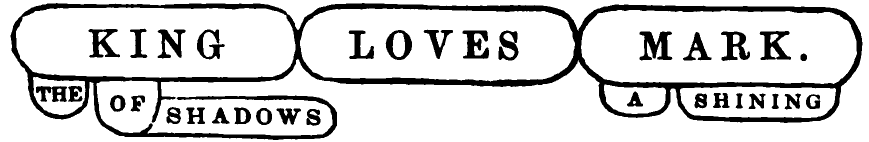
\includegraphics[width=.75\textwidth]{figures/04/Clark.png}
    \caption{Sample bubble diagram \citep[23]{Clark1847}\label{fig:4:3}}
\end{figure}

In \figref{fig:4:3}, which depicts the analysis of \REF{ex:4:2}, horizontally arranged bubbles express that the sentence is a combination of a \is{subject} subject, a \is{predicate}predicate and, optionally, an \is{object}object. These elements can be complemented by\is{adjuncts}adjuncts, which are represented by vertically connected bubbles. Note that adjuncts can also have adjuncts of their own: the representational convention is recursive. As it can be observed at the bottom left of the diagram, the representation of the terms of prepositional phrases combines two ways of aggregating bubbles. \is{Prepositional phrases}\text{Prepositional phrases} are a combination of a preposition (called the \textit{leader} in Clark’s terminology) and a noun (the \textit{subsequent}). The leader is represented by a bubble that connects vertically to the word the phrase complements, and is horizontally arranged with its subsequent.

Similar ideas were adopted in the manuals written by A. Reed and B. Kellogg, albeit with alternate graphical means of expressing the analyses. As already highlighted in \sectref{sec:4:2.2}, \figref{fig:4:2}b is a diagram containing words reified by labeled strokes that aggregate with one another. The sentence is a combination of a \is{subject}subject, a \is{predicate}predicate and, optionally, an \is{object}object. It is represented by horizontally arranged strokes. These elements can be complemented by \is{modifiers}modifiers, which are reified by vertically connected strokes. \is{Prepositional phrases}\text{Prepositional phrases} are a combination of a preposition and a noun: a vertically connected stroke for the preposition, which in turn is horizontally arranged with the noun. 

\subsection{Continuity between \citet{Clark1847} and \citet{ReedBrainerd1879}}\label{sec:4:3.2}

The theoretical assumptions in \citet{Clark1847} and \citet{ReedBrainerd1879} are roughly the same: both systems acknowledge a distinction between principal parts and adjuncts/modifiers, and posit a hybrid status for prepositional phrases. From a graphical perspective, both systems reify words by means of labeled geometric shapes that aggregate with one another either horizontally or vertically. Such similarities demonstrate some continuity between the diagramming systems. Additionally, there was a huge variety of diagramming systems that were proposed by different authors between Clark’s grammar and the \textit{Graded lessons of English} of Reed and Kellogg. Many of them relied on variations of the same principles, demonstrating the popularity of Clark’s ideas. \figref{fig:4:4} illustrates this with diagrams collected by \citet[37, 56, 75]{Brittain1973}.

\begin{figure}
    \begin{subfigure}[t]{\linewidth}\centering
	    \caption{\citealt[153]{Chandler1862}}
	  	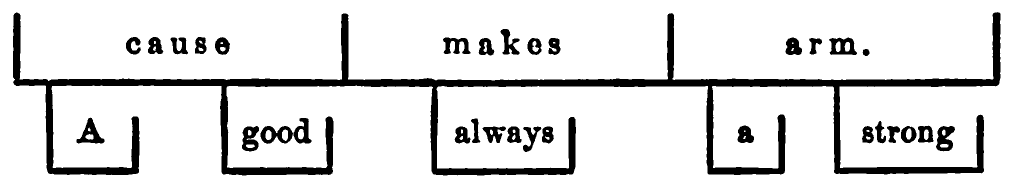
\includegraphics[width=0.75\textwidth]{figures/04/Chandler.png}
    \end{subfigure}\medskip\\%
    \begin{subfigure}[t]{\linewidth}\centering
	    \caption{\citealt[265]{Burtt1869}}
	  	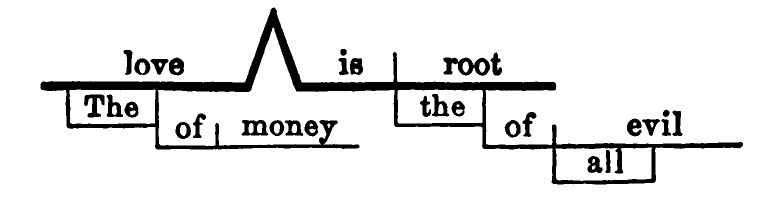
\includegraphics[width=0.75\textwidth]{figures/04/Burtt.png}
    \end{subfigure}\medskip\\%
    \begin{subfigure}[t]{\linewidth}\centering
	    \caption{\citealt[51]{Lighthall1872}}
	  	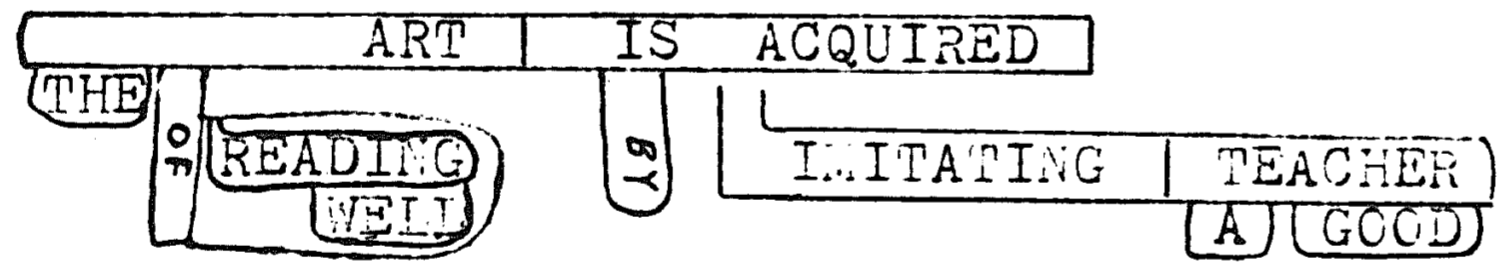
\includegraphics[width=0.75\textwidth]{figures/04/Lighthall.png}
    \end{subfigure}
    \caption{Various diagrams\label{fig:4:4}}
 \end{figure}

It is striking that each author chooses a different geometric shape to reify words, but the way the entities are arranged remains mostly identical as far as the basic structures are concerned (horizontal arrangement of the principal parts and vertical arrangement of the \is{adjuncts}adjuncts). The core descriptive stance of these diagrams is \textit{sparsity}: whenever it is possible, only the words are reified, and any other piece of information is expressed by configurational conventions.

Bubbles, open boxes, closed boxes, and strokes are theoretically equivalent. However, strokes are mono-dimensional entities, whereas bubbles and boxes are bi-dimensional ones. The initial choice of basic entities has consequences for the depiction of more complex constructions. This will be demonstrated in \sectref{sec:4:4} by comparing Clark’s system to the one developed by Reed and Kellogg.

\section{The logic of space: Case studies}\label{sec:4:4}

In the following subsections, I will study the graphical means at use to represent three kinds of syntactic relations in Clark’s system and in Reed \& Kellogg’s diagrams, namely: the relation between the subject and the predicate (\sectref{sec:4:4.1}), coordination (\sectref{sec:4:4.2}) and subordination of the subject (\sectref{sec:4:4.3}). All three relations somewhat break the sparsity of Reed \& Kellogg’s model by introducing additional entities.

\subsection{Subject-predicate relation}\label{sec:4:4.1}

A fundamental relation that every syntactic diagramming system has to depict is the one that holds between the \is{subject}subject and the \is{predicate}predicate. This relation has already been illustrated in §§\ref{sec:4:2.2} and~\ref{sec:4:3.1}.

\begin{figure}
    (a) \hspace{1em} 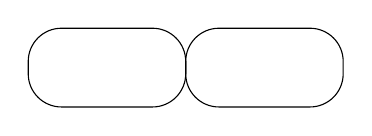
\begin{tikzpicture}[baseline=(current bounding box.center)]
    \draw [rounded corners=12pt] (0,0) rectangle (2,1); 
    \draw [rounded corners=12pt] (4,0) rectangle (2,1);
    \end{tikzpicture}
    \hspace{2cm}
    (b) \hspace{1em} 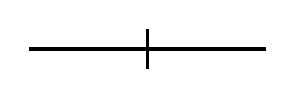
\begin{tikzpicture}[baseline=(current bounding box.center)]
    \draw [very thick] (0,0) -- (3,0); 
    \draw [very thick] (1.5,-.25) -- (1.5,.25);
    \end{tikzpicture}
    \caption{Visual models for the subject-predicate relation. (a) Clark; (b) Reed \& Kellogg.\label{fig:4:5}}
\end{figure}


\figref{fig:4:5}a is a \textit{visual model}: it represents the configurational rules in Clark’s grammar: Clark simply connects two bubbles from left to right. Bubbles clearly delimit their perimeters without any possibility of confusion, and their relative positions are sufficient to express the role of the words they contain. Therefore, only the words that are reified and only two entities are necessary.

In Reed \& Kellogg’s approach, the stroke corresponding to the subject and the one corresponding to the predicate in the graphical model (\figref{fig:4:5}b) could not have been joined by a mere concatenation. Because of the mono-dimensionality of the strokes, the resulting configuration would have been a single line, with no means of distinguishing between syntactic roles. Reed and Kellogg understood this shortcoming only too well:

\begin{quote}
I will draw on the board a heavy, or shaded, line, and divide it into two parts [. . . ]. I will consider the first part as a sign of the \is{subject}subject of a sentence, and the second part as a sign of the \is{predicate}predicate of a sentence. (\citealt[17]{ReedBrainerd1879})
\end{quote}

They use a vertical dash to part the subject from the predicate, which yields the model in \figref{fig:4:5}b. From a visual point of view, this vertical dash is an additional entity that does not correspond to a word. Paradoxically, using a graphical device to \textit{separate} two units creates an entity that corresponds to the grammatical relation that \textit{unites} them. For this reason, three entities are necessary: one for the \is{subject}subject (a horizontal stroke), one for the \is{predicate}predicate (a second horizontal stroke), and a third one for the relation between the subject and the predicate (a vertical dash).

The hierarchy between the subject-predicate relation and the predicate-object relation is not obvious in Clark’s diagrams, nor in the text that accompanies the diagrams.\footnote{ \textrm{See \citet[§4.3.2]{ImrenyiMazziotta2020}.}} Some diagrams that contain a subject and a predicate as well as an object were interpreted by some contemporary authors \citep[30]{Jewell1867} in a way that conceptualizes equivalent structural positions. By contrast, diagrams such as \figref{fig:4:6} suggest a visual hierarchy. Reed \& Kellogg state several times that the \textit{object complements} “complete” the predicate: “You will see that the line standing for the \is{object}\textit{object complement} is a continuation of the \is{predicate}predicate line, and that the little vertical line only touches this without cutting it” (\citealt[54]{ReedBrainerd1879}).

\ea \label{ex:4:3} Fulton invented the first steamboat.\z

 \begin{figure}
     (a) \hspace{1em} \begin{minipage}[c]{.45\textwidth}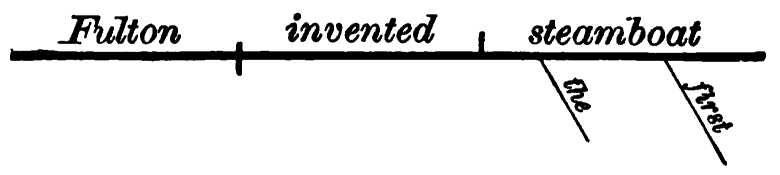
\includegraphics[width=\textwidth]{figures/04/ReedKellog2.png}\end{minipage}\hfill
     (b) \hspace{1em} 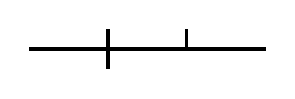
\begin{tikzpicture}[baseline=(current bounding box.center)]
    \draw [very thick] (0,0) -- (3,0); 
    \draw [very thick] (1,-.25) -- (1,.25);
    \draw [very thick] (2,0) -- (2,.25);
    \end{tikzpicture}
     \caption{Objects in Reed \& Kellogg’s system: (a) \citeyear[53]{ReedBrainerd1879}; (b) Visual model.\label{fig:4:6}}
 \end{figure}


Again, the use of a stroke to separate the verb from the object complement is actually an entity that reifies the relation that unites them. This graphical convention corresponds to a hierarchical analysis whereby the object is part of the predicate. This ICA-like analysis is related to the entities used to render the words and their relations: aggregated bubbles alone would allow for such a reification of part-whole relations only by inclusion.

\subsection{\is{Coordination}Coordination}\label{sec:4:4.2}

Traditional grammatical theory posits that coordination adds complexity to syntactic structures by allowing for several units to share the same grammatical role.\footnote{\textrm{Some modern approaches prefer to assume that the conjuncts have asymmetric syntactic roles. This difference is expressed by the way the conjuncts are encoded in the syntactic structure – see \citet{Mouret2007} for such examples in constituent trees and \citet[50--51]{PolguereMeltschuk2009} for an example of asymmetric dependency-based description.}} 

\begin{figure}
    (a) \hspace{1em} \begin{minipage}[c]{.45\textwidth}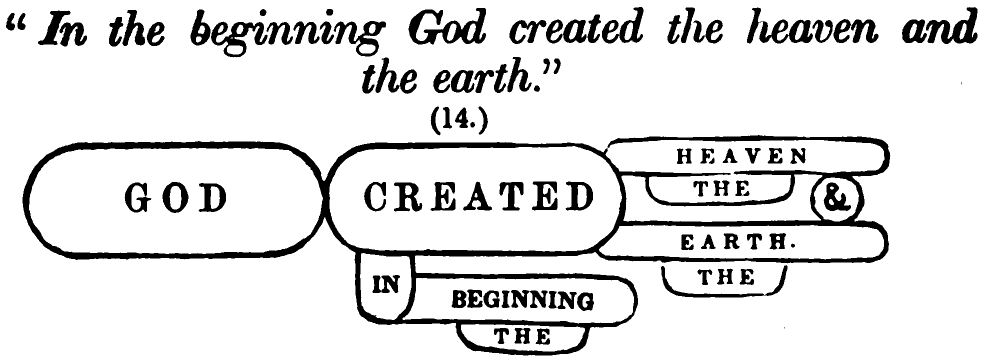
\includegraphics[width=\textwidth]{figures/04/Clark2.png}\end{minipage}\hfill
    (b) \hspace{1em} \begin{tikzpicture}[baseline=(current bounding box.center)]
    \node (n1) [draw, rounded corners=12pt, minimum width=1.5cm, minimum height=3cm, inner sep=0pt] at (0,0) {}; 
    \node (n2) [right=1cm of n1.north east, anchor=north,draw, rounded corners=12pt, minimum width=2cm, minimum height=1cm, inner sep=0pt] {}; 
    \node (n3) [right=1cm of n1.south east, anchor=south,draw, rounded corners=12pt, minimum width=2cm, minimum height=1cm, inner sep=0pt] {};
    \node (n4) [right=1.75cm of n1.center, anchor=center, draw, circle, minimum size=1cm, inner sep=0pt] {}; 
    \end{tikzpicture}
    \caption{Coordination in Clark’s system: (a) \citet[24]{Clark1847} (b) Visual model.\label{fig:4:7}}    
\end{figure}
 



In Clark’s system, words that are coordinated aggregate with the surrounding bubbles in the same way as they would if they were not. In \figref{fig:4:7}a, \textit{the heaven} and \textit{the earth} are both objects of the predicate \textit{created}, and they are connected to it horizontally. The \is{coordinative conjunction}\text{coordinative conjunction and} unites them by aggregating vertically with both. Should the conjunction be absent, Clark would use the symbol ‘×’ to express that it is implied. The model in \figref{fig:4:7}b provides a synthesis of the entities at use: there are four of them, one for each word. The bi-dimensionality of the bubbles makes them extensible vertically and horizontally. Therefore, the size of the bubbles may be altered to facilitate the marking of connections with no change in their values.\footnote{\textrm{\textsuperscript{} }\textrm{There are several other examples of such alteration in Clark’s work and most of them are coordinations.} } 


\begin{figure}
    (a) \hspace{1em} \begin{minipage}[c]{.75\textwidth}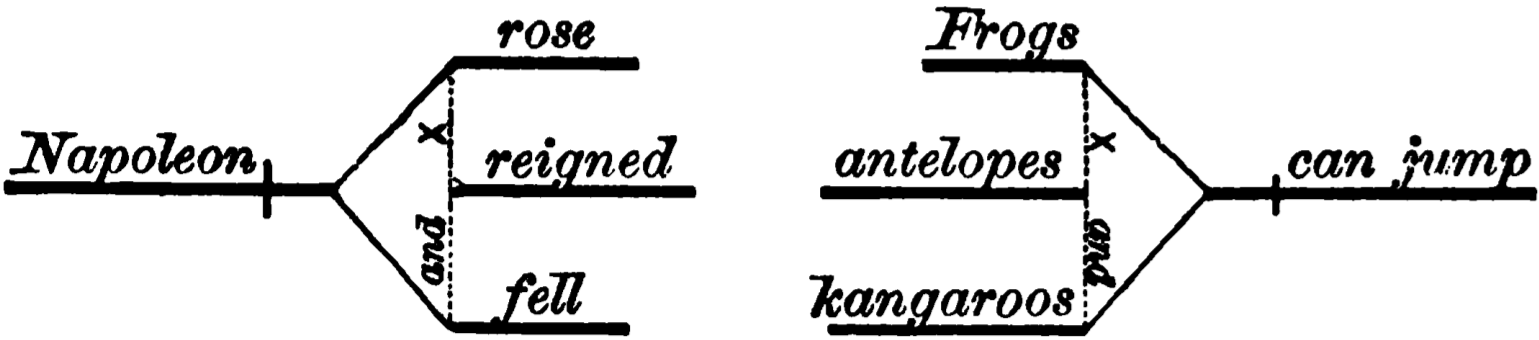
\includegraphics[width=\textwidth]{figures/04/ReedKellog3.png}\end{minipage}\bigskip\\
    (b) \hspace{1em} 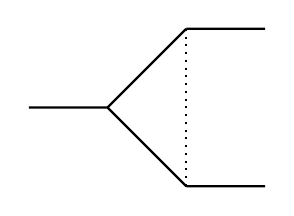
\begin{tikzpicture}[baseline=(current bounding box.center)]
                         \draw[thick] (0,0) -- (1,0)
                                      (1,0) -- (2,1)
                                      (2,1) -- (3,1)
                                      (1,0) -- (2,-1)
                                      (2,-1)-- (3,-1);
                          \draw[dotted,thick] (2,1) -- (2,-1);                                      
                     \end{tikzpicture}
    \caption{Coordination in Reed \& Kellogg’s system: (a) \citeyear[47]{ReedBrainerd1879}; (b) Visual model.\label{fig:4:8}}    
\end{figure}


The mono-dimensional strokes of the diagrams by Reed and Kellogg do not have the same properties: the only ways they can be manipulated is by changing their thickness (which does not really add another dimension), their slope, or their continuity (using dots instead of a continuous line). They cannot be extended vertically. Therefore, the authors had to create a device to represent coordinations. They describe the first example given in \figref{fig:4:8}a as follows:

\begin{quote}
The short line following the subject line represents the entire predicate, and is supposed to be continued in the three horizontal lines that follow, each of which represents one of the parts of the compound predicate. These lines are united by dotted lines, which stand for the connecting words. The × denotes that an \textit{and} is understood. (\citealt[47--48]{ReedBrainerd1879})
\end{quote}

The graphical model of coordination in \figref{fig:4:8}b shows that the number of strokes exceeds the number of nodes. The slanted lines, which are thinner than the horizontal ones, represent the part-whole relation between a syntactic unit taken as a whole and its component (the conjuncts). The notation integrates three additional entities that aggregate with the words: two of them are used to represent the part-whole relation, and the third one represents the larger syntactic unit. In the case of coordination, using strokes with a specific slope offers no other solution but to introduce additional entities: one for each part-whole relation between the conjuncts and the group they form, and, of course, one for this very group.

\subsection{Subordinate clauses as subjects}\label{sec:4:4.3}

\is{Subordinate clauses}\text{Subordinate clauses} are not handled in a consistent way either, in Clark’s grammar  (see \citealt[319--322 and 328--329]{Mazziotta2016}) or in the diagrams by Reed and Kellogg. Adjunct clauses are not represented with the same graphical conventions as the ones introduced by complementizers as \is{objects}objects or as \is{subjects}subjects.\footnote{ \textrm{This may be due to the heterogeneous treatment of dependents of the verb, since neither Clark nor Reed \& Kellogg overtly acknowledge verb-centrality (\sectref{sec:4:4.1}).}} I will focus on the latter, which Clark names “auxiliary sentences”. Auxiliary clauses assert “dependent proposition[s]” (\citeyear[187]{Clark1870}).

\ea \label{ex:4:4} That good men sometimes commit faults cannot be denied. \z

\begin{figure}
     (a) \hspace{1em} \begin{minipage}[c]{.45\textwidth}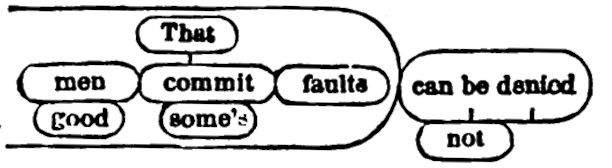
\includegraphics[width=\textwidth]{figures/04/Clark3.png}\end{minipage}\medskip\\
     (b) \hspace{1em} \begin{tikzpicture}[baseline=(current bounding box.center)]
                           \node (n1) [draw, rounded corners=12pt, minimum width=2cm, minimum height=1cm, inner sep=0pt, outer sep=3pt] at (0,0) {}; 
                           \node (n2) [draw, rounded corners=12pt, minimum width=2cm, minimum height=1cm, inner sep=0pt, outer sep=3pt] at (2,0) {};
                           \draw [rounded corners=12pt] (n1.north west) -- (n2.north) -- (n2.north east) -- (n2.south east) -- (n1.south west);
                           \node (n3) [right=0pt of n2,draw, rounded corners=12pt, minimum width=2cm, minimum height=1cm, inner sep=0pt] {};
                      \end{tikzpicture}
    \caption{Subordinate subject in Clark’s system: (a) \citeyear[47]{Clark1870}; (b) Visual model.\label{fig:4:9}}
\end{figure}
 

In \figref{fig:4:9}a, the subject clause, \textit{that good men sometimes commit faults} is wrapped in half an ellipsis that represents an abstract \is{subject}subject – I will not comment on the position of the complementizer. The spatial configuration that expresses the relation between the subject and the predicate (cf. \sectref{sec:4:4.1}) is not sufficient to represent complex structures that are used as \is{subjects}subjects: the subordinate \is{predicate}predicate \textit{commit} is already aggregated to the right of the subject \textit{men}, and to the left of the object \textit{faults}. There is no room left to its right for another \is{predicate}predicate, for the structure would then concatenate five bubbles without any means of distinguishing the predications from one another. The introduction of an additional entity establishes a hierarchy between the predications. It does so by a specific configuration: an inclusion layout that is made possible by the bi-dimensionality of the entity. There are two important consequences to this choice of representation: (i) the part-whole relations between the subject and its constituents are iconic; (ii) the combination of this wrapping bubble with the predicate \textit{can be denied} operates exactly in the same way as if it were a single word.

Due to the mono-dimensionality of the lines, the corresponding representation by Reed \& Kellogg does not use inclusion.

\ea \label{ex:4:5} That stars are suns is taught by astronomers. \z


\begin{figure}
     (a) \hspace{1em} \begin{minipage}[c]{.45\textwidth}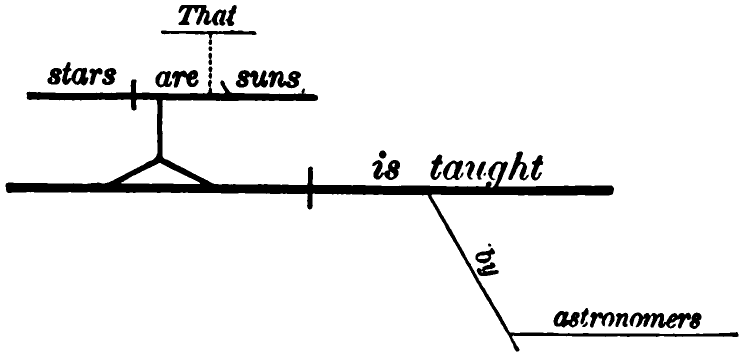
\includegraphics[width=\textwidth]{figures/04/ReedKellog4.png}\end{minipage}\medskip\\
     (b) \hspace{1em} \begin{tikzpicture}[baseline=(current bounding box.center)]
                      \draw [thick] (0,0) -- (4,0)
                                    (2,-.15) -- (2,.15);
                      \draw (1.25,0) -- (1.5,.15) -- (1.75,0);
                      \draw (1.5,.15) -- (1.5,1.5)
                            (0,1.5) -- (2,1.5)
                            (1.25,1.65) -- (1.25,1.35);                   
                      \end{tikzpicture}
    \caption{Subordinate subject in Reed \& Kellogg’s system: (a) \citeyear[81]{ReedBrainerd1879}; (b) Visual model.\label{fig:4:10}}
\end{figure}

The description of the diagram in \figref{fig:4:10}a clearly identifies a special device used as a “support” for the subordinate clause: “As this [sentence] subject cannot, in its proper form, be written on the subject line, it is placed above, and, by means of a support, the [sentence] diagram is made to rest on the subject line” (\citealt[107]{ReedBrainerd1879}).

Since the configurational rationales of the combination between the subject and the predicate are the same as in Clark’s system (horizontal connection), it follows that lines offer no other possibility but to introduce an additional entity in such cases. This entity could have been a wrapping device much as Clark’s or a connecting entity. Reed \& Kellogg chose the latter. The mono-dimensionality of strokes does not allow the depicting of inclusion in an iconic way. As a result, what is expressed by this entity is a relation of equivalence between the abstract subject and its realization as a clause – interestingly, the subordinate clause is connected via its predicate to the abstract subject.

\section{Conclusions}\label{sec:4:5}

Diagrams are graphical means of representing syntactic analyses. There are several ways to visually represent words and analytic concepts. The first distinction is between \textit{entities} and \textit{spatial configuration}: as shown in \sectref{sec:4:2.2}, grammarians may choose to represent relations between words with entities that reify them (\figref{fig:4:2}a) or by their layout (\figref{fig:4:2}b). When different grammarians choose to reify the same units, they may use different entities to express similar analyses (cf. \sectref{sec:4:3}). However, the material choice of different shapes (bubbles in the case of Clark, and strokes for Reed \& Kellogg) as diagrammatic entities has consequences for the spatial configuration of the entities, and on the amount of entities needed to express the analyses. In the case of the relation between the subject and the predicate, Clark could use a simple configurational convention at his disposal to arrange the bubbles representing a subject and a predicate, whereas Reed \& Kellogg had to introduce an additional entity. In an indirect way, this additional entity can be interpreted as a representation of the relation between the subject and the predicate. Similar means can be used to identify the verb-object relation, thus leading to a model that decomposes the sentence into two strata of relations (cf. \sectref{sec:4:4.1}). A related issue concerns the representation of coordinate constructions: since conjuncts share the same positions in the syntactic structure, diagrams should represent this feature. With bi-dimensional entities, it is possible to do so in an iconic way, whereas the use of strokes implies the use of additional entities that reify abstract units representing the combination of the conjuncts (cf. \sectref{sec:4:4.2}). The representation of subordinate subjects (or objects) also implies the introduction of abstract entities in all kinds of diagrams, be they a wrapping entity or a connecting one (cf. \sectref{sec:4:4.3}). 

From these observations, it appears that diagrams making use of mono-di\-men\-sio\-nal objects are less minimalistic. The use of mono-dimensional strokes forces to reify abstract units that are not words, but rather represent part-whole relations or the integrity of complex structures considered as wholes. Indeed, current constituent trees (\figref{fig:4:1}) constantly and consistently represent this kind of syntactic arrangement. A similar tendency was already developing at the time when Alonzo Reed and Brainerd Kellogg were drawing their first diagrams.

Graphical entities chosen to express the analyses always constrain what kind of relations can be represented. More often than not, they imply the creation of \textit{artefacts}, i.e. graphical objects that are not part of the knowledge transmitted by the analysis, but entirely pertain to the graphical formalism that encodes it.

% % \section*{Acknowledgements}

{\sloppy\printbibliography[heading=subbibliography,notkeyword=this]}
\end{document}
